\section{Combinatorial Encoding by the $\mathrm{O}$-Matrix}\label{sec:combinatorics}

For a simple affine arrangement of $n$ lines, choose a generic directed line
$\gamma$ (the \emph{sweep line}) that is not parallel to any line of the
arrangement and whose initial position is sufficiently far from all
intersection points. Label the lines $L_0,L_1,\dots,L_{n-1}$
(or simply $0, 1, \dots, n-1$) in the order in which
$\gamma$ meets them at its initial position. As $\gamma$ sweeps
through the plane, each intersection point $L_i\cap L_j$ is encountered
exactly once; append~$j$ to the row of~$L_i$ and~$i$ to the row of~$L_j$
at that moment. The result is an $n\times(n-1)$ matrix
which we call the $\mathrm{O}$-matrix (order matrix) of the arrangement.

The numbering $L_0,L_1,\dots,L_{n-1}$ induced by $\gamma$ coincides with the
increasing angular order of the lines; the same numbering is used in the
parameter tables and figures throughout the paper.

This construction applies to pseudoline arrangements as well; in that case
the $\mathrm{O}$-matrix encodes the same data as a rank-$3$ oriented matroid
(equivalently, an allowable sequence of permutations).
We use the $\mathrm{O}$-matrix since its row-based format is convenient: each row
directly records the sequence of crossings along a line, while adjacency of
labels within rows detects bounded faces.

\begin{figure}[ht]
\centering
\definecolor{triEdgeA}{RGB}{220,38,38}
\definecolor{triEdgeB}{RGB}{56,163,28}
\definecolor{triEdgeC}{RGB}{136,48,212}
\newcommand{\edgeacolor}[1]{\textcolor{triEdgeA}{\mathbf{#1}}}
\newcommand{\edgebcolor}[1]{\textcolor{triEdgeB}{\mathbf{#1}}}
\newcommand{\edgeccolor}[1]{\textcolor{triEdgeC}{\mathbf{#1}}}
\begin{minipage}[t]{0.32\linewidth}

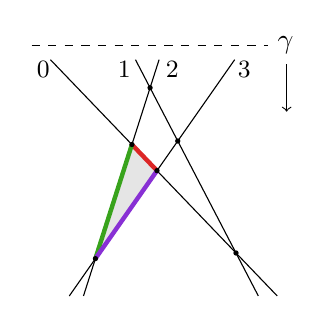
\begin{tikzpicture}[scale=1.2,baseline=2.9cm]
  \coordinate (L1a) at (-0.8,2.5);
  \coordinate (L1b) at (1.6,0);
  \coordinate (L2a) at (0.1,2.5);
  \coordinate (L2b) at (1.4,0);
  \coordinate (L3a) at (0.35,2.5);
  \coordinate (L3b) at (-0.45,0);
  \coordinate (L4a) at (1.15,2.5);
  \coordinate (L4b) at (-0.6,0);
  % Compute all intersection points
  \coordinate (P12) at (intersection of L1a--L1b and L2a--L2b);
  \coordinate (P13) at (intersection of L1a--L1b and L3a--L3b);
  \coordinate (P14) at (intersection of L1a--L1b and L4a--L4b);
  \coordinate (P23) at (intersection of L2a--L2b and L3a--L3b);
  \coordinate (P24) at (intersection of L2a--L2b and L4a--L4b);
  \coordinate (P34) at (intersection of L3a--L3b and L4a--L4b);
  % Shaded triangle: (l0, l2, l3)
  \fill[gray!20] (P13) -- (P14) -- (P34) -- cycle;
  % Draw lines with labels at pos along the line
  \draw (L1a) -- (L1b) node[pos=0.04,left,font=\small]{$0$};
  \draw (L2a) -- (L2b) node[pos=0.04,left,font=\small]{$1$};
  \draw (L3a) -- (L3b) node[pos=0.04,right,font=\small]{$2$};
  \draw (L4a) -- (L4b) node[pos=0.04,right,font=\small]{$3$};
  % Highlight the three sides of the triangle with matching colors
  \draw[triEdgeA, line width=1.6pt] (P13) -- (P14);
  \draw[triEdgeB, line width=1.6pt] (P13) -- (P34);
  \draw[triEdgeC, line width=1.6pt] (P14) -- (P34);
  % Intersection points
  \foreach \p in {P12,P13,P14,P23,P24,P34}
    \fill (\p) circle (0.8pt);
  % Sweep line gamma (horizontal, moving downward)
  \draw[dashed] (-1.0,2.65) -- ++(2.5,0) node[right]{$\gamma$}
    ++(0.2,-0.2) edge[solid, ->] ++(0,-0.5);
\end{tikzpicture}
\end{minipage}%
\hfill
\begin{minipage}[t]{0.32\linewidth}
$\mathrm{O}$-matrix

\medskip
\renewcommand{\arraystretch}{1.2}
$\begin{array}{c|ccc}
  & 1\text{st} & 2\text{nd} & 3\text{rd} \\
\hline
  L_0 & \edgeacolor{2} & \edgeacolor{3} & 1 \\
  L_1 & 2 & 3 & 0 \\
  L_2 & 1 & \edgebcolor{0} & \edgebcolor{3} \\
  L_3 & 1 & \edgeccolor{0} & \edgeccolor{2}
\end{array}$

\end{minipage}
\hfill
\begin{minipage}[t]{0.32\linewidth}
\raggedright
\setlength{\baselineskip}{1.22\baselineskip}
The shaded triangle $(L_0,L_2,L_3)$ corresponds to
the adjacent pairs:\\
$\edgeacolor{2},\edgeacolor{3}$ in row~$L_0$;\;\\
$\edgebcolor{0},\edgebcolor{3}$ in row~$L_2$;\;\\
$\edgeccolor{0},\edgeccolor{2}$ in row~$L_3$.
\end{minipage}
\caption{A simple arrangement of four lines, its $\mathrm{O}$-matrix, and the
correspondence between faces and adjacency in the matrix.}
\label{fig:omatrix-example}
\end{figure}

\begin{lemma}[$\mathrm{O}$-matrix criterion for bounded faces]\label{lem:face-criterion}
Let $(L_{i_1},\dots,L_{i_k})$ be a cyclically ordered list of distinct
pseudolines in a simple arrangement. Then
these pseudolines bound a bounded $k$-gonal face if and only if for every
$s=1,\dots,k$ (with $i_0=i_k$ and $i_{k+1}=i_1$)
the two labels $i_{s-1}$ and $i_{s+1}$ appear in adjacent positions in the row
of $L_{i_s}$ of the $\mathrm{O}$-matrix:
$$
\mathrm{O}[i_s] = (\dots, i_{s\pm1}, i_{s\mp1}, \dots),
\qquad s=1,\dots,k.
$$
\end{lemma}

\begin{proof}
Along $L_{i_s}$, the segment between $L_{i_s}\cap L_{i_{s-1}}$ and
$L_{i_s}\cap L_{i_{s+1}}$ is an edge of a bounded face precisely when it
contains no other crossing, i.e., $i_{s-1}$ and $i_{s+1}$ are adjacent in the
row of $L_{i_s}$. Imposing this for every $s$ gives a closed polygonal
boundary.
\end{proof}
